% Desenvolvido por: Prof. Dr. David Buzatto
%
% Versão 1.6.2
% Data: 21/12/2022

\documentclass[
	article,
	11pt,
	oneside,
	a4paper,
	chapter=TITLE,
	section=TITLE,
	english,
	brazil,
	sumario=tradicional
]{abntex2}

\usepackage{estrutura}
\usepackage[brazilian,hyperpageref]{backref}
\usepackage[alf,abnt-emphasize=bf]{abntex2cite}

% ---
% Dados do documento
% ---

\tipotrabalho{Artigo}

\titulo{Título}
\instituicao{Instituto Federal de Educação, Ciência e Tecnologia de São Paulo}
\campus{São João da Boa Vista}
\area{Área de Concentração do Trabalho}

\aluno{Nome Completo}
\local{São João da Boa Vista}

\dia{DIA}
\mes{MÊS}
\ano{ANO}

\curso{Nome do Curso}
\grau{Definição do grau}

%exemplos
%\curso{Tecnologia em Sistemas para Internet}
%\grau{Tecnólogo em Sistemas para Internet}
%\curso{Especialização em Desenvolvimento de Aplicações para Dispositivos Móveis}
%\grau{Especialista em Desenvolvimento de Aplicações para Dispositivos Móveis}

\orientador{Prof./Profa. Esp./Me./Dr./Dra. Nome Completo Orientador}
\gradorientador{Nome do Curso de Graduação do Orientador}
\instgradorientador{Nome da Instituição da Graduação do Orientador}
\posorientador{Especialista/Mestre/Doutor em Nome do Curso de Pós-graduação do Orientador}
\instposorientador{Nome da Instituição da Pós-graduação do Orientador}
\docorientador{Curso Superior em que o Orientador da Aulas majoritariamente}

% caso não haja coorientador, comente as próximas seis linhas
\coorientador{Prof./Profa. Esp./Me./Dr./Dra. Nome Completo Coorientador}
\gradcoorientador{Nome do Curso de Graduação do Coorientador}
\instgradcoorientador{Nome da Instituição da Graduação do Coorientador}
\poscoorientador{Especialista/Mestre/Doutor em Nome do Curso de Pós-graduação do Coorientador}
\instposcoorientador{Nome da Instituição da Pós-graduação do Coorientador}
\doccoorientador{Curso Superior em que o Coorientador da Aulas majoritariamente}

% exemplo
%\orientador{Prof. Dr. David Buzatto}
%\gradorientador{Sistemas de Informação}
%\instgradorientador{UniFEOB}
%\posorientador{Doutor em Biotecnologia}
%\instposorientador{UNAERP}
%\docorientador{Tecnologia em Sistemas para Internet}

%\coorientador{Prof. Dr. Breno Lisi Romano}
%\gradcoorientador{Ciência da Computação}
%\instgradcoorientador{UNIFEI}
%\poscoorientador{Doutor em Engenharia Eletrônica e Computação}
%\instposcoorientador{ITA}
%\doccoorientador{Tecnologia em Sistemas para Internet}

\definirdata
\definirautores

\makeindex

\setlrmarginsandblock{3cm}{3cm}{*}
\setulmarginsandblock{3cm}{3cm}{*}
\checkandfixthelayout
\setlength{\parindent}{1.3cm}
\setlength{\parskip}{0.2cm}
\setlength{\ABNTEXcitacaorecuo}{1.8cm}
\SingleSpacing

% ----
% Início do documento
% ----
\begin{document}
	
	% Seleciona o idioma do documento
	\selectlanguage{brazil}
	
	% Retira espaço extra obsoleto entre as frases.
	\frenchspacing 
	
	% ----------------------------------------------------------
	% ELEMENTOS PRÉ-TEXTUAIS
	% ----------------------------------------------------------
	
	% Se desejar escrever o artigo em duas colunas, descomente a linha abaixo
	% e a linha com o texto "FIM DE ARTIGO EM DUAS COLUNAS".
	% \twocolumn[    		% INICIO DE ARTIGO EM DUAS COLUNAS
    
	% título
	\maketitle
    
	% resumo em português
	\begin{resumoumacoluna}
		
		Neste trabalho é apresentada a formatação que deve ser utilizada nos artigos a serem submetidos ao final dos cursos de Graduação e Pós-Graduação do IFSP câmpus São João da Boa Vista. Leia com atenção este documento. O máximo de palavras para o resumo é 250 (duzentos e cinquenta). 
		
		\vspace{\onelineskip}
		
		\noindent
		\textbf{Palavras-chave}: Palavra-chave 1. Palavra-chave 2. Palavra-chave 3. Palavra-chave n.
		
	\end{resumoumacoluna}
	
    % resumo em inglês
    \renewcommand{\resumoname}{Abstract}
    \begin{resumoumacoluna}
    	
        \begin{otherlanguage*}{english}
   	    	Resumo em inglês.
   		
       		\vspace{\onelineskip}
   		
   	    	\noindent
   		   \textbf{Keywords}: Keyword 1. Keyword 2. Keyword 3. Keyword n.
   		   
      \end{otherlanguage*} 
  
   	\end{resumoumacoluna}
        
	% ]  				% FIM DE ARTIGO EM DUAS COLUNAS
	
	% ----------------------------------------------------------
	% ELEMENTOS TEXTUAIS
	% ----------------------------------------------------------
	\textual
	
	% ----------------------------------------------------------
	% Introdução
	% ----------------------------------------------------------
	\section{Introdução}
	
    Neste documento estão listadas as seções obrigatórias que você deverá fornecer, bem como os exemplos dos comandos mais comuns que serão utilizados na construção de seu documento. Para pesquisar sobre mais comandos, recomenda-se a utilização do site \url{https://ctan.org/}, que é a biblioteca principal do \LaTeX, e o do site \url{https://tex.stackexchange.com} que é uma das principais comunidades para solução de dúvidas relacionadas a \LaTeX. Ambas são em inglês.	
    
    
%%%%%%%%%%%%%%%%%%%%%%%%%%%%%%%%%%%%%%%%%%%%%%%%%%%%%%%%%%%%%%%%%%

	\section{Desenvolvimento}
    	
     Texto do desenvolvimento.
     
     
     
     %%%%%%%%%%%%%%%%%%%%%%%%%%%%%%%%%%%%%%%%%%%%%%%%%%%%%%%%%%%%%
     
     \subsection{Revisão da Literatura}
     
     Texto da revisão da literatura.
     
     Este é um exemplo de como usar figuras. Referência cruzada: Figura~\ref{fig:exemplo}
     
     \FloatBarrier
     \begin{figure}[!htbp]
     	\centering
     	\caption{Exemplo de figura}
     	%scale redimensiona a figura.
     	%1.5 = 150% do tamanho original
     	%1 = 100% do tamanho original
     	%0.20 = 20% do tamanho original
     	
\includegraphics[scale=1.5]{imagens/exemploFigura}
     	\\\textbf{Fonte:} Elaborada pelo autor
     	\label{fig:exemplo}
     \end{figure}
     \FloatBarrier
     
     
     Este é um exemplo de como usar tabelas. Referência cruzada: Tabela~\ref{tab:exemplo}
     
     \FloatBarrier
     \begin{table}[!htbp]
     	\centering
     	\caption{Exemplo de tabela de 2 colunas}
     	\begin{tabular}{ c | c }
     		\hline
     		\textbf{Coluna 1} & \textbf{Coluna 2} \\ \hline
     		Dado 1a           & Dado 2a           \\ \hline
     		Dado 1b           & Dado 2b           \\ \hline
     		Dado 1c           & Dado 2c           \\ \hline
     		Dado 1d           & Dado 2d           \\ \hline
     	\end{tabular}
     	\\ \vspace{0.2cm}
     	\textbf{Fonte:} Elaborada pelo autor
     	\label{tab:exemplo}
     \end{table}
     \FloatBarrier
     
     
     Este é um exemplo de como usar quadros. Referência cruzada: Quadro~\ref{qua:exemplo}
     
     \FloatBarrier
     \begin{quadro}[!htbp]
     	\centering
     	\caption{Exemplo de quadro}
     	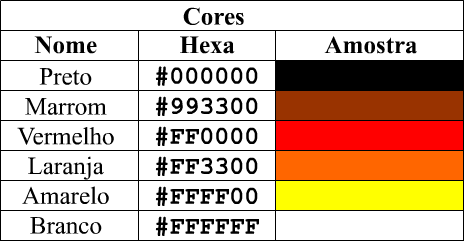
\includegraphics[scale=.7]{imagens/exemploQuadro}
     	\\\textbf{Fonte:} Elaborada pelo autor
     	\label{qua:exemplo}
     \end{quadro}
     \FloatBarrier
     
     
     Este é um exemplo de como usar equações. Referência cruzada: Equação~\ref{eq:exemplo}
     
     \begin{equation}
     \sum_{i=1}^{n} i = \frac{n(n+1)}{2}
     \label{eq:exemplo}
     \end{equation}
     
     
     Exemplo de inserção de lista de código fonte:
     
     \lstinputlisting[language=Java]{fontes/ClasseExemplo.java} 
     
     
     
     Este é um exemplo de como inserir texto sem formatação (ambiente verbatim):
     
     \begin{verbatim}
     Texto sem formatação, como espaçamento igual.
     \end{verbatim}
     
     
     Exemplo de lista de itens:
     
     \begin{itemize}
     	\item \textbf{Item 1:} texto...;
     	\item \textbf{Item 2:} texto...;
     	\begin{itemize}
     		\item \textbf{Subitem:} texto...;
     		\item \textbf{Subitem:} texto...;
     		\item \textbf{Subitem:} texto...;
     	\end{itemize}
     	\item \textbf{Item 3:} texto...;
     	\item \textbf{Item n:} texto....
     \end{itemize}
     
     
     Exemplo de lista numerada:
     
     \begin{enumerate}
     	\item \textbf{Item:} texto...;
     	\item \textbf{Item:} texto...;
     	\begin{enumerate}
     		\item \textbf{Subitem:} texto...;
     		\item \textbf{Subitem:} texto...;
     		\item \textbf{Subitem:} texto...;
     	\end{enumerate}
     	\item \textbf{Item:} texto...;
     	\item \textbf{Item:} texto....
     \end{enumerate}
     
     
     Exemplos de comandos para texto e referências:
     
     \begin{itemize}
     	\item Para iniciar um novo parágrafo, basta deixar uma linha em branco no código fonte;
     	\item Não force o compilador a pular mais de uma linha, pois terá influência negativa na composição do documento;
     	\item Sempre deixe o \LaTeX\ realizar a formatação de parágrafos e posicionamento de elementos;
     	\item Utilização de aspas simples (abertura \verb|`|, fechamento \verb|'|): `Texto entre aspas simples';
     	\item Utilização de aspas duplas (abertura \verb|``|, fechamento \verb|''|): ``Texto entre aspas duplas'';
     	\item Negrito (comando \verb|\textbf|): \textbf{texto em negrito};
     	\item Itálico (comando \verb|\textit|): \textit{texto em itálico};
     	\item Sublinhado (comando \verb|\underline|): \underline{texto sublinhado};
     	\item Negrito e itálico (usar comandos juntos): \textbf{\textit{texto em negrito e itálico}};
     	\item Alterar cor do texto (comando \verb|\textcolor{cor}{texto}|):
     	\begin{itemize}
     		\item Exemplo \verb|\textcolor{red}{texto}|: \textcolor{red}{texto vermelho};
     		\item Exemplo \verb|\textcolor[RGB]{255, 102, 0}|: \textcolor[RGB]{255, 102, 0}{texto laranja};
     		\item Exemplo \verb|\textcolor[HTML]{006AD7}|: \textcolor[HTML]{006AD7}{texto azul};
     	\end{itemize}
     	\item Ambiente matemático inline (comando \verb|$ expressão $|): $s = x^2-2x +1$;
     	\item Referência normal (comando \verb|\cite|):
     	\begin{itemize}
     		\item \cite{Agaisse1995};
     		\item \cite{Abedi2014};
     		\item \cite{BtNomenclature2016};
     	\end{itemize}
     	\item Referência normal com mais de uma obra (comando \verb|\cite|):
     	\begin{itemize}
     		\item \cite{Abedi2014, Agaisse1995};
             \item \cite{AgapitoTenfen2014, BtNomenclature2016, Nelson2014};
     	\end{itemize}
     	\item Referência nome e ano (comando \verb|\citeauthorandyear|):
     	\begin{itemize}
     		\item \citeauthorandyear{Agaisse1995};
     		\item \citeauthorandyear{Abedi2014};
     		\item \citeauthorandyear{BtNomenclature2016};
     	\end{itemize}
     \end{itemize}
     
     
     Exemplo 1 de citação direta:
     
     \begin{citacao}
     	Os 20 aminoácidos usualmente encontrados como resíduos em proteínas contém um grupo $\alpha$-carboxil, um grupo $\alpha$-amino e um grupo R distinto substituído no átomo de carbono $\alpha$. O átomo de carbono $\alpha$ de todos os aminoácidos, com exceção da glicina, é assimétrico e, portanto, os aminoácidos podem existir em pelo menos duas formas estereoisoméricas. Somente os estereoisômeros L, com uma configuração relacionada à configuração absoluta da molécula de referência L-gliceraldeído, são encontrados em proteínas \cite[p. 81]{Nelson2014}.
     \end{citacao}
     
     Exemplo 2 de citação direta:
     
     \begin{citacao}
     	\textit{These various insecticidal proteins are synthesized during the stationary phase and accumulate in the mother cell as a crystal inclusion which can account for up to 25\% of the dry weight of the sporulated cells. The amount of crystal protein produced by a B. thuringiensis culture in laboratory conditions (about 0.5 mg of protein per ml) and the size of the crystals (24) indicate that each cell has to synthesize $10^6$ to $2 \times 10^6$ $\delta$-endotoxin molecules during the stationary phase to form a crystal} \cite[p. 1]{Agaisse1995}.
     \end{citacao}
     
     Exemplo de nota de rodapé\footnote{Essa é uma nota de rodapé!}.
     
     
     \subsubsection{Trabalhos Correlatos}
     
     Pesquise e descreva no mínimo três trabalhos correlatos ao seu.
     
     \subsubsubsection{Trabalho 1}
     
     Texto...
     
     \subsubsubsection{Trabalho 2}
     
     Texto...
     
     \subsubsubsection{Trabalho 3}
     
     Texto...
     
     %%%%%%%%%%%%%%%%%%%%%%%%%%%%%%%%%%%%%%%%%%%%%%%%%%%%%%%%%%%%%
     
     \subsection{Metodologia}
     
     Texto da metodologia.
     
     
     
     %%%%%%%%%%%%%%%%%%%%%%%%%%%%%%%%%%%%%%%%%%%%%%%%%%%%%%%%%%%%%
     
     
%%%%%%%%%%%%%%%%%%%%%%%%%%%%%%%%%%%%%%%%%%%%%%%%%%%%%%%%%%%%%%%%%%

	\section{Resultados e Discussão}
    	
     Texto dos resultados.
     
     
     
%%%%%%%%%%%%%%%%%%%%%%%%%%%%%%%%%%%%%%%%%%%%%%%%%%%%%%%%%%%%%%%%%%

	\section{Conclusões/Conclusões parciais}
	
	Texto das conclusões. Lembre-se de apontar possíveis trabalhos futuros.
	
	\textbf{Obs:} Esta seção deve ser intitulada ``Conclusões Parciais'' em trabalhos de graduação para a Validação de Projeto de TCC. Na Avaliação Final de TCC o nome da seção deve ser ``Conclusões''.
    
    
    
%%%%%%%%%%%%%%%%%%%%%%%%%%%%%%%%%%%%%%%%%%%%%%%%%%%%%%%%%%%%%%%%%%

	\section{Cronograma}
	
	Segue abaixo o cronograma das atividades que serão executadas até a Avaliação Final de TCC.
	
	\textbf{Obs:} Para facilitar, crie o cronograma usando o modelo do Word contido no projeto (imagens/templateCronograma.docx), ou qualquer outro \textit{software}, salve a imagem e atualize o arquivo imagens/cronograma.png.
	
	\FloatBarrier
	\begin{figure*}[!htbp]
		\centering
		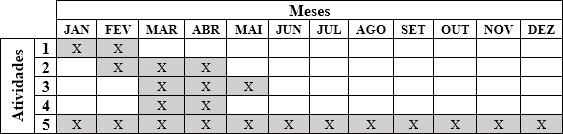
\includegraphics[scale=1]{imagens/cronograma}
	\end{figure*}
	\FloatBarrier
	
	\begin{enumerate}
		\item Descrição da atividade 1;
		\item Descrição da atividade 2;
		\item Descrição da atividade 3;
		\item Descrição da atividade 4;
		\item Descrição da atividade 5.
	\end{enumerate}
	
	\textbf{Obs:} Esta seção deve ser elaborada e estar contida em trabalhos de graduação para a Validação de Projeto de TCC. Na Avaliação Final de TCC esta seção não deve existir, visto que não haverá atividades após a Avaliação Final.
	
	
	% ----------------------------------------------------------
	% ELEMENTOS PÓS-TEXTUAIS
	% ----------------------------------------------------------
	\postextual
	\bibliography{referencias}
	
	%
    % Este é um exemplo da ata de defesa.
    %
    % A ata de defesa será fornecida pelo professor orientador após a defesa do trabalho
    % e o orientado será responsável em substituir o arquivo de exemplo pelo arquivo final.
    %
    \begin{folhadeaprovacao}
    	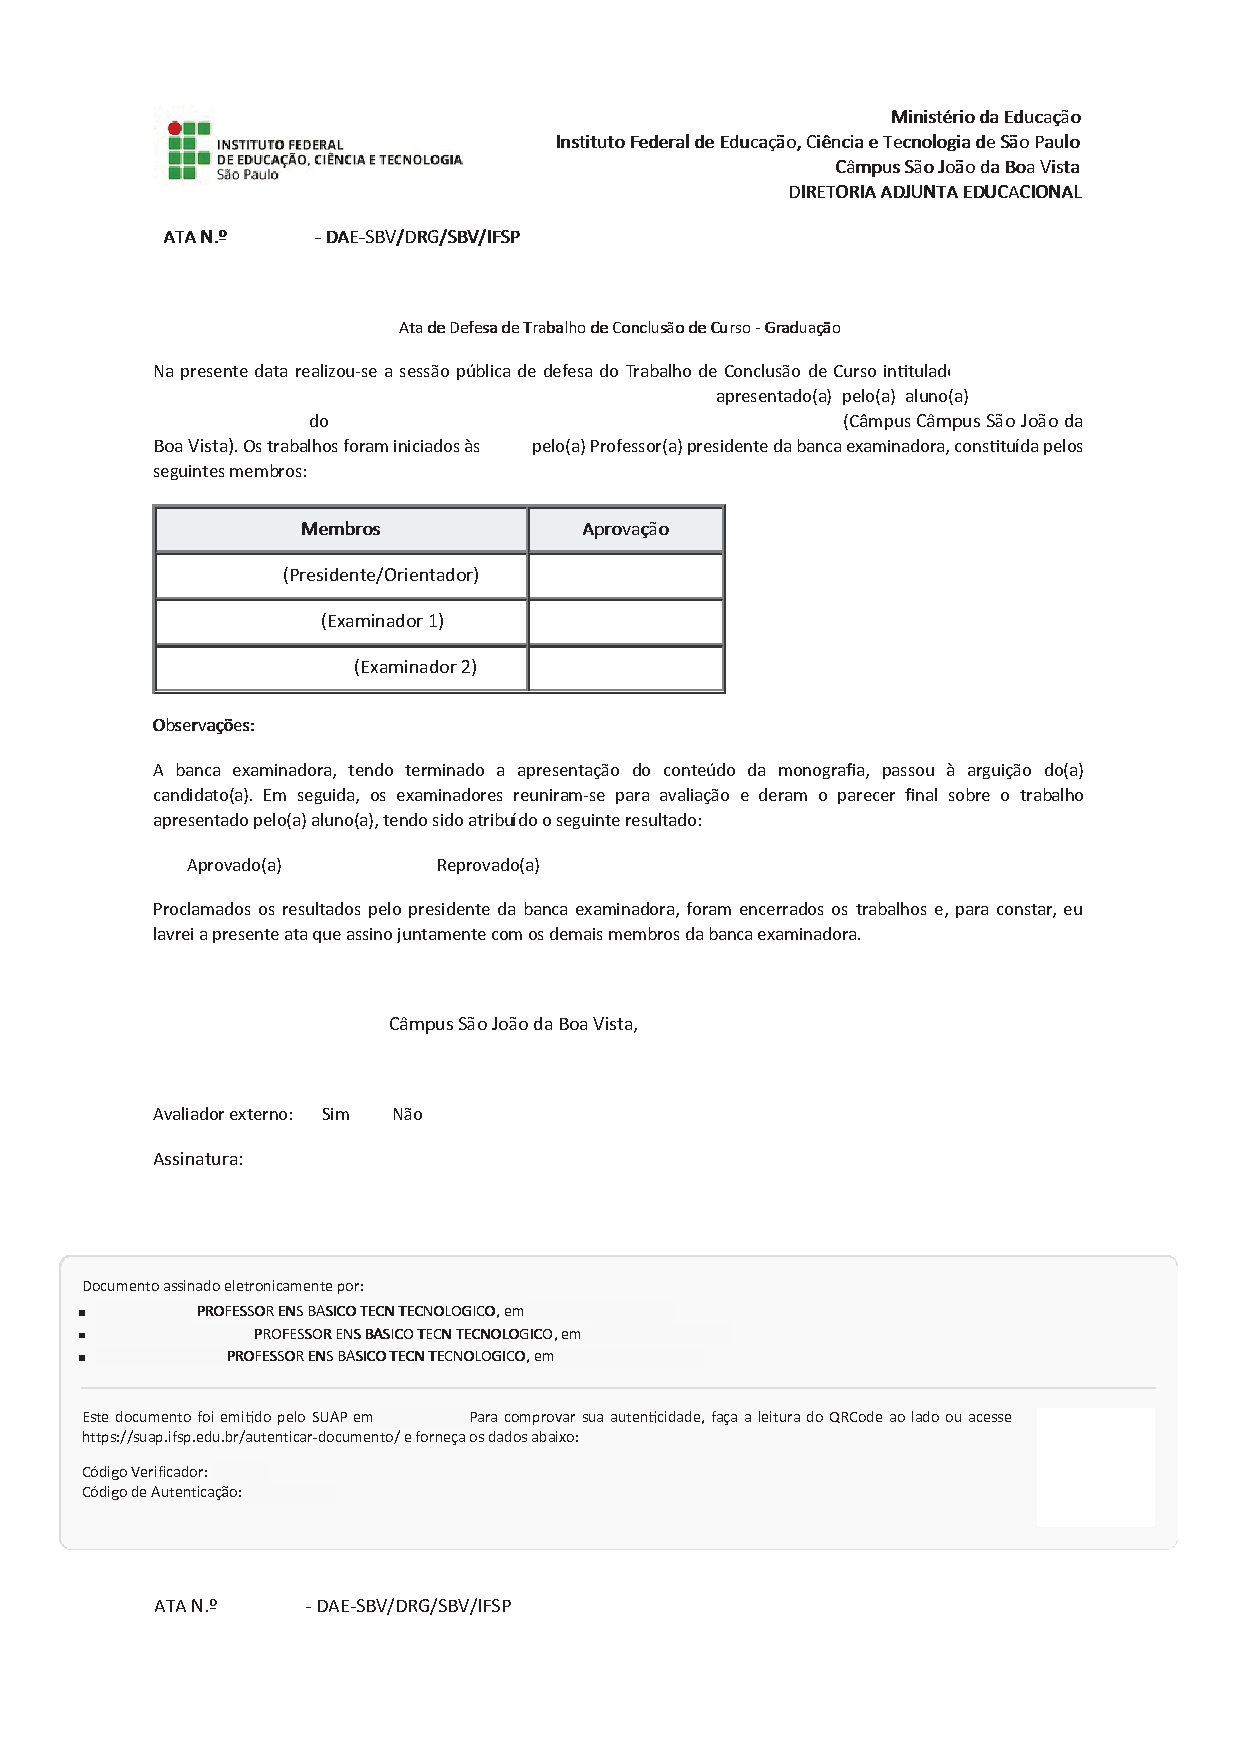
\includepdf[pages={1-}]{ataDefesa/exemploAtaDefesa.pdf}
    \end{folhadeaprovacao}

\end{document}